%\documentclass[12pt,twoside,titlepage,сa4paper]{article}
\documentclass[specialist,
               substylefile = spbu.rtx,
               subf,href,colorlinks=true, 12pt]{disser}

\usepackage[a4paper,
            mag=1000, includefoot,
            left=3cm, right=1.5cm, top=2cm, bottom=2cm, headsep=1cm, footskip=1cm]{geometry}
\usepackage[utf8]{inputenc}
\usepackage[english, russian]{babel}
% \usepackage{csquotes}
\usepackage[defaultmono]{droidmono}
\usepackage[T2A]{fontenc}


\usepackage[intlimits]{amsmath}
\usepackage{amsfonts}
\usepackage{amssymb}
\usepackage{amsthm}

\usepackage{algorithm2e}
\usepackage{graphicx}
\graphicspath{ {media/} }
\usepackage{listings}
\usepackage{color}

\usepackage[fixlanguage]{babelbib}
\selectbiblanguage{russian}

% \usepackage{natbib}
% \usepackage[backend=biber,style=numeric]{biblatex}
% \addbibresource{biblio-u.bib}

% \usepackage{statmodtitle}
% \usepackage[top=1in,bottom=1in,left=1in,right=1in]{geometry}
\usepackage{hyperref}
\newtheorem{theorem}{Теорема}
\newcommand{\ev}{\mathsf{E}}
\newcommand{\R}{\ensuremath{\mathbb{R}}}

\renewcommand\topfraction{0.85}
\renewcommand\bottomfraction{0.85}
\renewcommand\textfraction{0.1}
\renewcommand\floatpagefraction{0.85}

% \title{Устранение экспоненциальной сложности оценки стоимости бермудского опциона}
% \author{Анастасия Миллер}
%\date{СПбГУ, 6${}^{\mbox{\small ой}}$ семестр,~~ 322 гр. \\ \today}
% \facility{Кафедра статистического моделирования}
% \supervisor{д.ф.-м.н.~Ермаков С.М.}

\setlength\parindent{0pt}
\setlength\parskip{0.5em}

\lstdefinestyle{customjava}{
%   belowcaptionskip=1\baselineskip,
  	breaklines=true,
  	breakatwhitespace=true,
%   xleftmargin=\parindent,
%   language=Java,
%   showstringspaces=false,
   	basicstyle=\footnotesize\fdmfamily,
   	keywordstyle=\bfseries\color{blue},
  	commentstyle=\color{magenta},
  	morekeywords={ImitatedAsset, },
  	% identifierstyle=\color{green},
%   stringstyle=\color{orange},
}
\lstset{style=customjava, language=Java}

\begin{document}
\institution{%
    Министерство образования и науки Российской Федерации \\
    Федеральное агентство по образованию \\
    Федеральное государственное образовательное учреждение высшего
    профессионального образования «Санкт-Петербургский государственный университет» \\
    Математико-механический факультет \\
    Кафедра статистического моделирования
}

% \apname{д.\,ф.-м.\,н., профессор С.\,М.~Ермаков}

\title{Отчёт о научно-исследовательской практике}

\topic{\normalfont\scshape %
Устранение экспоненциальной сложности оценки стоимости бермудского опциона}

\author{Миллер Анастасия Александровна}

\sa {С.\,М.~Ермаков}
\sastatus{д.\,ф.-м.\,н., профессор}

\city{Санкт-Петербург}
\date{\number\year}

\maketitle

% \institution{
% 	Saint Petersburg State University \\
% 	Faculty of Mathematics and Mechanics \\
% 	Department of Statistical Modelling
% }

% % \apname{Professor S.\,M.~Ermakov}

% \title{Graduation Thesis Report}

% \topic{\normalfont\scshape
%     Elimination of exponential complexity in Bermudian option pricing}

% \author{Miller Anastasia}

% \sa {S.\,M.~Ermakov}
% \sastatus{Professor}

% % \rev {A.\,Y.~Shlemov}
% % \revstatus{PhD student}

% \city{Saint Petersburg}
% \date{\number\year}


% \maketitle[en]
\tableofcontents

\intro
	\par Метод оценки американских опционов с конечным числом дат погашения, основанный на моделировании дерева событий (метод случайных деревьев), был предложен в \citep{Glasserman2004} ещё в 2004 году. Этот метод моделирует изменение состояния базового актива через случайные деревья, разветвляющиеся в каждой из возможных дат раннего погашения опциона. При анализе деревьев могут быть получены две оценки: смещённая вверх и смещённая вниз, являющиеся асимптотически несмещёнными и дающие доверительный интервал для истинной цены опциона.
	\par Вычислительная сложность этих оценок --- $O\left( b^s \right)$, где $b$ --- количество ветвей дерева (моделируемых вариантов изменения цены опциона), $s$ --- количество шагов алгоритма (дат погашения опциона). Рассмотрим реализацию и анализ одного из способов снизить вычислительную сложность этих оценок.

\chapter{Алгоритм}
	\par Рассматриваем опцион с $s$ датами исполнения, общий период времени положим равным 1, т.е.\ имеем $\left\lbrace t_k \right\rbrace _{k=1}^s$ --- набор моментов времени. Смоделированное состояние актива (на который выписан опцион) в момент времени $t_k$ описывается $Ы_k^{i_1 \cdots i_k}$, где $\forall\, k \in 1:s\quad i_k \in 1:b$ ($i_j$ указывает на номер узла, выбранный на $j$-ом шаге).
	
	\par Начиная с некоторого момента $t_k$, когда общее число состояний на шаге достигнет некоторого $n$, мы перестанем генерировать дочерние вершины ко всем состояниям. В следующий момент времени, $t_{k+1}$, мы будем иметь всё так же $n$ состояний, а не $bn$. 
	\par В том случае, когда состояние актива $S$ является числом в $\R ^1$, в качестве параметра $X$, распределение которого нас интересует, можно использовать  само $S$, иначе можно использовать $h(S)$. 
	\par Деля интервал $\left[\min_{i\in 1:n} X_i ; \max_{i\in 1:n} X_i + \frac{1}{n}\right)$ на $k$ равных частей $\left[a_{k-1},a_k\right)$, где $a_0 = \min_{i\in 1:n} X_i$, $a_k = \max_{i\in 1:n} X_i$, мы можем определить частоты \[f_k = \frac{1}{n}\#\left\lbrace X_i \middle\vert X_i\in\left[a_{k-1},a_k\right)\right\rbrace\] попадания событий в различные части отрезка. Из состояний, сгруппированных на отрезке $\left[a_{k-1},a_k\right)$, мы также можем создать некоторый <<средний арифметический>> вектор, кооринаты которого будут являться средним арифметическим координат всех состояний, оказавшихся на данном отрезке, и уже для этого нового среднего состояния --- представителя отрезка --- генерировать дочерние вершины в количестве $n\cdot f_k$. Для всех состояний, оказавшихся в этом отрезке, дочерними вершинами будут являться все вершины, полученные от их представителя. 
	\par Таким образом, количество рассматриваемых состояний не увеличится.
\chapter{Реализация}
	\par В качестве параметра, распределение которого будет анализироваться, я использовала цену актива (реализацию винеровского случайного процесса, где каждое следующее состояние получается из предыдущего как $p_0 \cdot (1 + a\cdot \bigtriangleup t + \sigma \cdot \varepsilon \cdot \sqrt{\bigtriangleup t})$, где $p_0$ --- цена актива в предыдущий момент времени, $\bigtriangleup t = 1/s$, $a$ и $\sigma$ означают доходность и волатильность цены акции соответственно и являются константами, $\varepsilon$ --- случайная величина со стандартным нормальным распределением).
	\par На рис.~\ref{fig:exponentialTree} можно видеть, как выглядит генерируемое исходным методом дерево.
	\begin{figure}[h]
		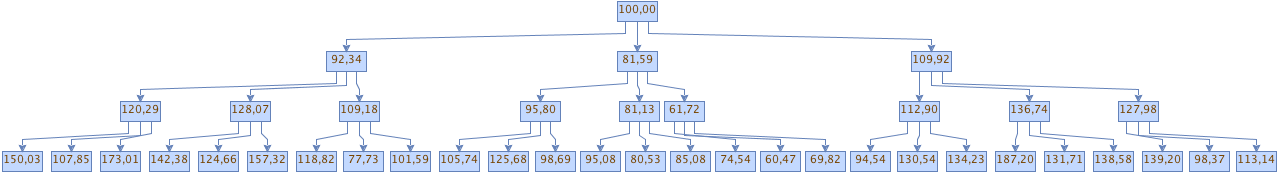
\includegraphics[width=\textwidth]{exp_tree}
		\caption{Дерево, генерируемое при использовании метода, описываемого Глассерманом (цифры в узлах --- стоимость актива)}
		\label{fig:exponentialTree}
	\end{figure}
	\par В своей реализации я разделяю генерацию дерева и подсчёт оценок, ему соответствующих, так как оценки, в отличие от исходных деревьев, у меня не отличаются от оценок у Броади и Глассермана. Вначале существовала надежда сравнивать <<полные>> и <<урезанные>> деревья, но она не оправдалась из-за слишком больших требований к памяти у классических деревьев.
	\par Момент, после которого стоит переходить на линейную модель генерации дочерних вершин, определился как $k = \left\lfloor ^{\log n} / _{\log b}\right\rfloor$ ($b$ --- количество ветвей у узла в <<экспоненциальном режиме>>, $n$ --- ширина дерева в <<линейном режиме>>). Реализацию можно увидеть в приложении \ref{lst:treeGeneration}.
	

	Дерево, генерируемое усечённым образом, можно увидеть на рис.~\ref{fig:linearTree}. 
	\begin{figure}%[h]
		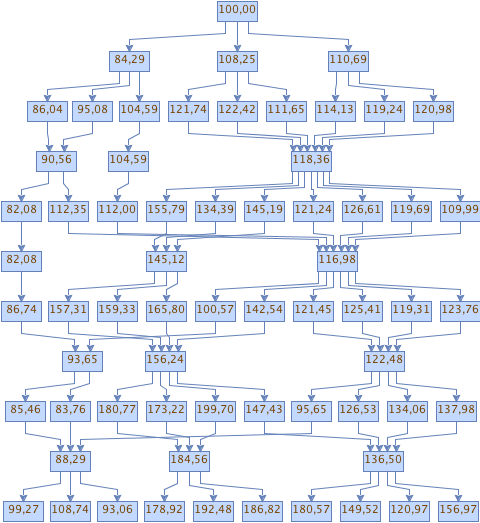
\includegraphics[width=0.9\textwidth]{linear_tree}
		\caption{Дерево, генерируемое усечённым методом (цифры --- стоимость актива; ширина дерева $n=10$, количество секторов $k=3$)}
		\label{fig:linearTree}
	\end{figure}
\chapter{Результаты}
	Целью увеличения доступного для обсчёта числа дат исполнения было максимально приблизиться к американскому опциону (опциону с возможностью исполнения в любой момент в оговорённом промежутке времени). Неизвестными факторами (поведение которых не было очевидным на стадии создания упрощённого метода) были ширина дерева $n$ и количество <<столбцов гистограммы>> $k$. Также было неясно, существует ли сходимость метода, сопоставимая со сходимостью исходного метода.
	\par Испытания сходимости метода были проведены по алгоритму \ref{alg:test}.
	% \begin{figure}[h]
	\begin{algorithm}
	\renewcommand{\AlCapSty}{\text}
	\SetAlgorithmName{Алгоритм}{алгоритм}{Список алгоритмов}
		\caption{Проверка сходимости оценки в испытании}
		\label{alg:test}
			\DontPrintSemicolon
			\SetKw{And}{and}
			startSteps = 50\;
			\For{$i \in 1:100$}{
				$x_1 = \infty$\;
				$x_0 = -\infty$\;
				step = 0\;
				\While{$\left|x_1-x_0\right| > \epsilon$ \And step<1000}{
					$x_0 = x_1$\;
					$x_1$ = estimateAsset(steps=startSteps+step, width=50, sectors=$k$)\;
					step += 1 \;
				}
				\eIf{step == 1000}{
					в этом испытании алгоритм не сошёлся
				}{
					в этом испытании алгоритм сошёлся
				}
			}
	\end{algorithm}
	% \end{figure}
	\par Для верхней оценки стоимости опциона результаты можно увидеть на рис.~\ref{fig:upperEstimate},
	\begin{figure}[h]
		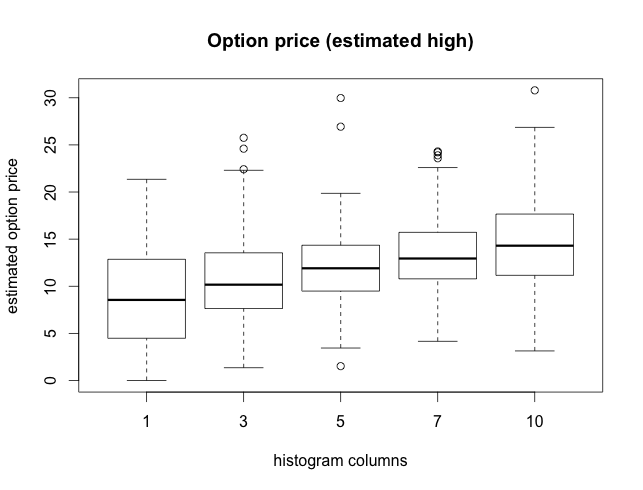
\includegraphics[width=\textwidth]{upper_estimate}
		\caption{Распределение верхней оценки стоимости опциона}
		\label{fig:upperEstimate}
	\end{figure}
	для нижней оценки --- на рис.~\ref{fig:lowerEstimate}.
	\begin{figure}[h]
		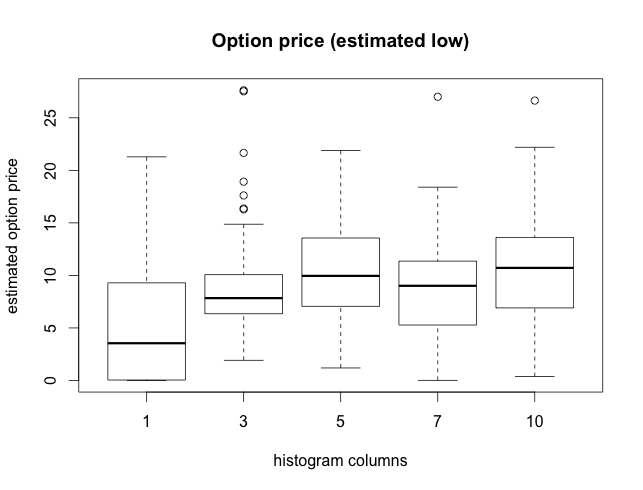
\includegraphics[width=\textwidth]{lower_estimate}
		\caption{Распределение нижней оценки стоимости опциона}
		\label{fig:lowerEstimate}
	\end{figure}

	Вероятность (выборочная) сходимости верхней и нижней оценки представлена на графиках \ref{fig:upperConvergence} и \ref{fig:lowerConvergence} соответственно.
	\begin{figure}[h]
		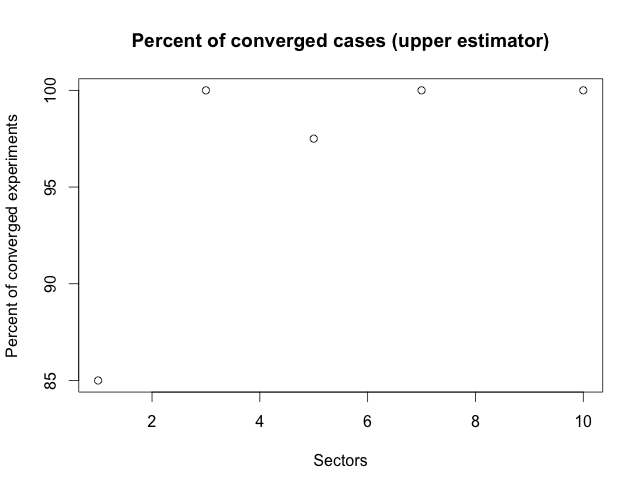
\includegraphics[width=\textwidth]{upper_convergence}
		\caption{Процент случаев, в которых верхняя оценка сошлась, по отношению к общему числу испытаний}
		\label{fig:upperConvergence}
	\end{figure}
	\begin{figure}[h]
		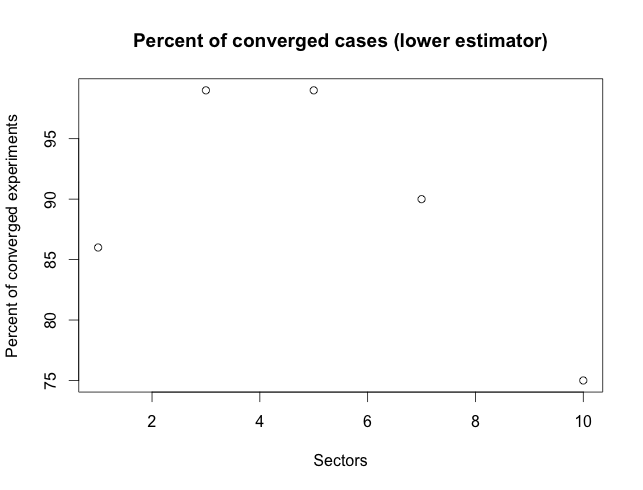
\includegraphics[width=\textwidth]{lower_convergence}
		\caption{Процент случаев, в которых нижняя оценка сошлась, по отношению к общему числу испытаний}
		\label{fig:lowerConvergence}
	\end{figure}

\conclusion
	Как видно, оценки имеют большую дисперсию, причём если для нижней оценки оптимальное разбиение на подмножества кажется равным 3 (для ширины в 50 узлов), то для верхней оценки локальный минимум не очевиден.

\section*{Дальнейшие планы}
	\begin{enumerate}
		\item Закончить рассмотрение оценки по гистограмме, в т.ч.\ найти аналитически математическое ожидание оценки (похожий случай уже рассмотрен в \citep{montekarlo1975})
		\item Рассмотреть оценку по кластерам (предполагаемый алгоритм кластеризации рассмотрен в \citep{Arthur2007})
		\item Рассмотреть другие оценки
	\end{enumerate}
\nocite{*}
\bibliographystyle{ugost2008}
\bibliography{biblio-u}

\appendix
\chapter{Реализация на Java}
\renewcommand{\lstlistingname}{Листинг}% Listing -> Algorithm
\renewcommand{\lstlistlistingname}{Листинги}
\begin{lstlisting}[caption={Генерирование дерева состояний актива, на который выписан опцион},label={lst:treeGeneration}]
public static ImitatedAsset generateAssetByHistogram(int width, int branch, int steps, int sectors, double initialPrice){
    timedelta = 1. / steps;
    int expSteps = (int) Math.floor(Math.log(width) / Math.log(branch));
    ImitatedAsset[] nodes = new ImitatedAsset[width];
    ImitatedAsset ans = generateTreeAssetsToModeling(branch, expSteps, initialPrice, nodes);

    ImitatedAsset[] new_nodes = generateFirstRow(width, sectors, nodes);
    nodes = new_nodes;

    // +1 because of one step that was done outside the cycle
    for (int step = expSteps + 1; step < steps; step++) {
        new_nodes = generateRow(width, (step + 1 == steps), sectors, nodes);
        nodes = new_nodes;
    }
    return ans;
}
private static ImitatedAsset[] generateRow(int width, boolean lastRow, int sectors, ImitatedAsset[] nodes) {
    ImitatedAsset[] new_nodes;
    sortArrayWithNulls(nodes);
    double sector = getSectorWidth(sectors, nodes);
    double min = extremalValue(nodes, -1);
    double sum = 0;
    int amount = 0;
    int k = 0;
    new_nodes = new ImitatedAsset[width];
    for (int j = 0; j < width; j++){ // iterating over {{nodes}}
        if (nodes[j].price > min + (k+1) * sector) { // reached the end of the sector
            generateBlock(nodes, new_nodes, lastRow, j-amount, j, amount, sum/amount);
            k++;
            amount = 0;
            sum = 0;
        }
        sum += nodes[j].price;
        amount++;
    }
    generateBlock(nodes, new_nodes, lastRow, width-amount, width, amount, sum/amount);
    return new_nodes;
}
private static void generateBlock(ImitatedAsset[] nodes, ImitatedAsset[] new_nodes, boolean lastRow, int start, int end, int children, double price, int new_start){
    ImitatedAsset asset = new ImitatedAsset(price, children, false); // intermediate asset will definitely have children
    for (int i = start; i < end; i++ ){ // assign average node as a child to the previous generation
        nodes[i].children[0] = asset;
    }
    for (int i = 0; i < children; i++){ // generating new nodes
        asset.children[i] = new ImitatedAsset(getRandomPrice(asset.price), 1, lastRow);
        new_nodes[new_start+i] = asset.children[i];
    }
}
	\end{lstlisting}

\end{document}